\documentclass[10 pt]{article}

\usepackage[top= 30mm, bottom=30mm, left=35mm, right=35mm]{geometry}
\usepackage[OT2]{fontenc}
\usepackage[serbian]{babel}
\usepackage{hyperref}
\usepackage{graphicx}
\usepackage{float}
\usepackage{caption}

\hypersetup{
    colorlinks=true,
    linktoc=all,
    linkcolor=blue,
}

\begin{document}
	
\begin{titlepage} 
	\centering 
	
	\rule{\textwidth}{1pt}
	
	\vspace{2pt}\vspace{-\baselineskip} 
	
	\rule{\textwidth}{0.4pt}
	
	\vspace{0.025\textheight}

	{\Huge Baza podataka za Stomatoloshku ordinaciju}
	
	\vspace{0.020\textheight}
	
	\rule{0.5\textwidth}{1pt}
	
	\vspace{0.5\textheight}
	
	\begin{minipage}{0.4\textwidth}
		\begin{flushleft} \large
			\emph{Autor:}\\
			Marija Mijailovic1 1093/2017
		\end{flushleft}
	\end{minipage}
	~
	\begin{minipage}{0.4\textwidth}
		\begin{flushright} \large
			\emph{Asistent:} \\
			Ivana Tanasijevic1
		\end{flushright}
	\end{minipage}\\[2cm]

	{\large \today}\\[2cm]
	
	\rule{1\textwidth}{1.5pt}
	
\end{titlepage}
	

\thispagestyle{empty}

\newpage
\renewcommand*\contentsname{Sadrzhaj:}
\tableofcontents

\newpage
\section{Opis baze}


\textbf{Stomatoloshka ordinacija} chuva sledec1e informacije:
\begin{itemize} 
	\item Pacijent(idPacijent, Ime, Prezime, DatumRodjenja, Adresa, Telefon, DatumOtvaranjaKartona, UkupanDug, Plac1eno, Napomena),
	\item ZatechenoStanje(idPacijent, Zub0-Zub31),
	\item Zaposleni(idZaposlenog, Ime, Prezime),
	\item Stomatolog(idStomatologa, Status, RadnoIskustvo),
	\item Tehnichar(idTehnichara, RadnoIskustvo), 
	\item Zub(idZub), 
	\item Materijal(idMaterijal, Naziv),
	\item Stolica(idOprema, BrojStolice), 
	\item Zahvat(shifra, idPacijent, Datum, idSpisak, idZub, idStomatolog,  idTehnichar) 
	\item SpisakIntervencija(idSpisak, NazivIntervencije, Cena, idOblastInt),
	\item OblastIntervencije(idOblastInt, NazivOblasti)
\end{itemize}

Zaposlen u ordinaciji mozhe biti Tehnichar ili Stomatolog, za Stomatologa se chuva josh i informacija o statusu zaposlenja, moguc1e vrednosti statusa zaposljenja bi bile: stalan radni odnos, privremen radni odnos, praksa i sl. 

Za svakog pacijenta se chuva informacija o njegovom zatechenom stanju svih zuba kada je prvi put doshao na pregled, i ti podaci se dalje ne menjaju. 
Svaki pacijent ima svoje zatecheno stanje.

Nad jednim pacijentom se mozhe obaviti vishe zahvata, dok jedan zahvat odgovara jednom pacijentu. Stomatolog mozhe da izvrshi jedan ili vishe zahvata nad pacijentom. Dok tehnichar mozhe , ali i ne mora da izvrshi zahvat nad pacijentom. Jedan zahvat se obavlja na jednoj stolici, dok na stolici mozhe biti obavljeno vishe zahvata, medjutim ne mora biti obavljen ni jedan. Za zahvat se chuva shifra zahvata i to je identifikacija zahvata, kako bi mogli da izvrshimo vishe zahvata u toku jednog dana nad istim pacijentom.  Prilikom zahvata pamtimo i nad kojim zubom je izvrshen zahvat. Nad jedinim zubom jednog pacijenta mozhe se izvrshiti vishe zahvata.

Svaki zahvat se nalazi na spisku intervencija. Spisak intervencija sadrzhi vishe zahvata, ali mora imati bar jedan zahvat. Svaki zahvat sa spiska intervencija pripada tachno jednoj oblasti. Za svaki zahvat sa Spiska intervencije se chuva i informacija koji je materijal potreban za taj zahvat. Jednoj intervenciji mozhe biti potrebno vishe materijala, dok jedan materijal se mozhe upotrebiti za vishe intervencija.

Odgovarajuc1i dijagram dat je na slici \ref{fig:dijagram}
\\
\\
\textbf{Zadovoljenost uslova:}
\begin{itemize}
	\item Nezavisni entiteti: Zaposleni, Pacijent, Stolica, OblastIntervencije, Materijal
	\item Agregirani entiteti: Obavlja, Koristi
	\item Zavisni entiteti: Zatecheno stanje
	\item Trigeri: 
		\begin{itemize}
			\item Nakon obavljene intervencije azhurira se dug pacijenta prema ordinaciji.
			\item Nakon odredjenog broja zahvata(npr.10) Zaposlenom se uvec1ava radno iskustvo za odredjeni broj(npr.20\%). 
		\end{itemize}	
\end{itemize}


\textbf{Upiti:}
\begin{enumerate}
	\item Izlistavanje svih zahvata odradjenih nad pacijentom(ime/prezime pacijenta se unosi sa standardnog ulaza).
	\item Unos novog zahvata(Nakon izlistanih svih zahvata datog pacijenta,bira se prvo oblast intervencije, zatim se izlistavaju intervencije koje pripadaju unetoj oblasti i bira se intervencija(idSpisak). Potom se unosi Datum kada je zahvat izvrshen, Zub nad kojim je izvrshen zahvat ili null, ako nije izvrsheno nad zubom vec1 nad aparatom(fiksnim ili pokretnim), i ko je izvrshio zahvat(tehnichar ili stomatolog). Pri ovom upitu se aktivira triger1 , i aktivirac1e se i triger 2 ako je broj zahvata zaposlenog vec1i od 10. 
	\item Azhuriranje podataka u okviru Pacijenta 
	\item Unos novog pacijenta(svi podaci se unose sa standardnog ulaza).
	\item Unos novog zatechenog stanja(svi podaci se unose sa standardnog ulaza).
	\item Brisanje Materijala, Pacijenta...
\end{enumerate}

\begin{figure}[H]
	\centering
	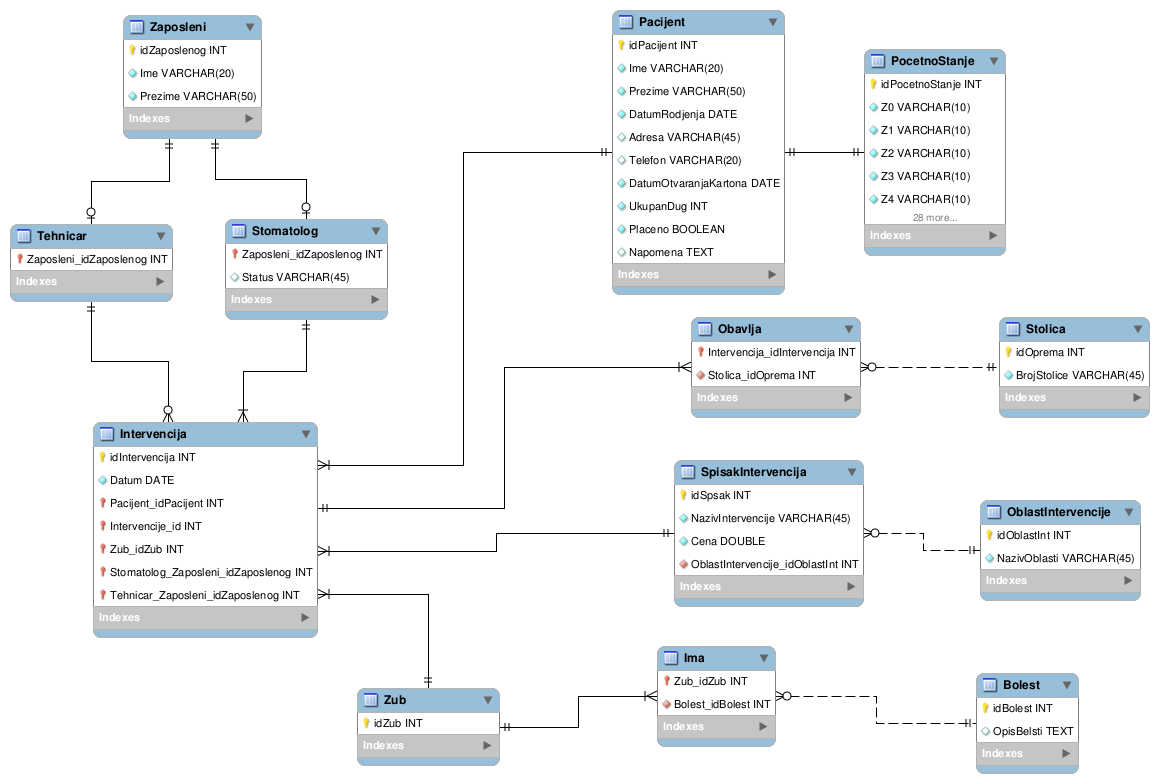
\includegraphics[width=15cm,height=15cm,keepaspectratio]{StomatoloskaOrdinacija.png}\\
	\caption{Stomatoloshka ordinacija \label{fig:dijagram}}
\end{figure}

\end{document} 